\documentclass[aspectratio=169, xcolor=table]{beamer}

\usepackage{calc}
\usepackage{graphicx}
\usepackage{mathtools}
\usepackage{siunitx}

\graphicspath{{./images}}
\setbeamertemplate{navigation symbols}{}

\author{Chris Doble}
\date{}
\subtitle{Building a GPS receiver from scratch}
\title{Part 7: Decoding}
\usetheme{Madrid}

% Show the topics frame at the start of each section
\AtBeginSection[]
{
  \begin{frame}
    \frametitle{Topics}
    \tableofcontents[currentsection, subsubsectionstyle=hide]
  \end{frame}
}

% Show the topics frame at the start of each subsection
\AtBeginSubsection[]
{
  \begin{frame}
    \frametitle{Topics}
    \tableofcontents[currentsection, currentsubsection, subsubsectionstyle=hide]
  \end{frame}
}

\begin{document}

\frame{\titlepage}

\begin{frame}
    \frametitle{Navigation message structure}

    \centering
    \begin{tabular}{ l|r|r }
        \textbf{Name} & \textbf{Number of bits} & \textbf{Emitted every} \\
        \hline
        Pseudosymbol & 1/20 & $\qty{1}{ms}$ \onslide<2-> \\
        Pseudobit / bit & 1 & $\qty{20}{ms}$ \onslide<3-> \\
        Word & 30 & $\qty{0.6}{s}$ \onslide<4-> \\
        Subframe & 300 & $\qty{6}{s}$ \onslide<5-> \\
        Frame & 1,500 & $\qty{30}{s}$
    \end{tabular}
\end{frame}

\section{Pseudosymbol integration}

\begin{frame}
    \frametitle{Pseudosymbol integration}

    \centering
    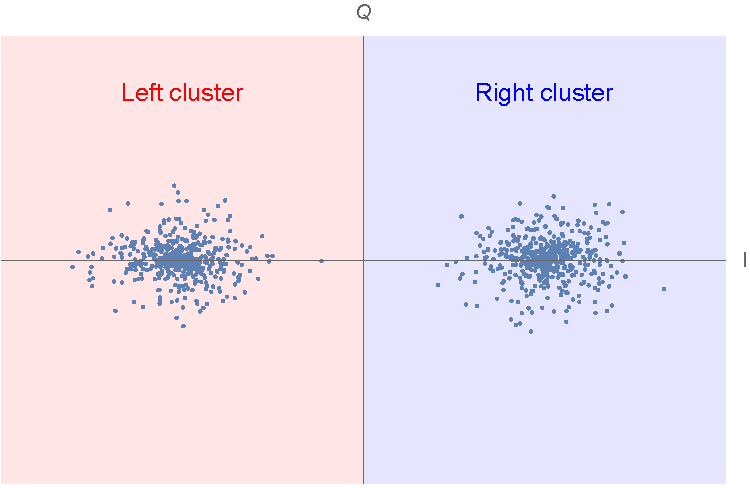
\includegraphics[width=\textwidth / 2]{1 correlations with regions.pdf}

    \Large
    \onslide<2->{\hspace{-0.5cm} $-1$ \hspace{2.75cm} $+1$}
\end{frame}

\begin{frame}
    \frametitle{Pseudosymbol integration}

    \centering
    \only<1>{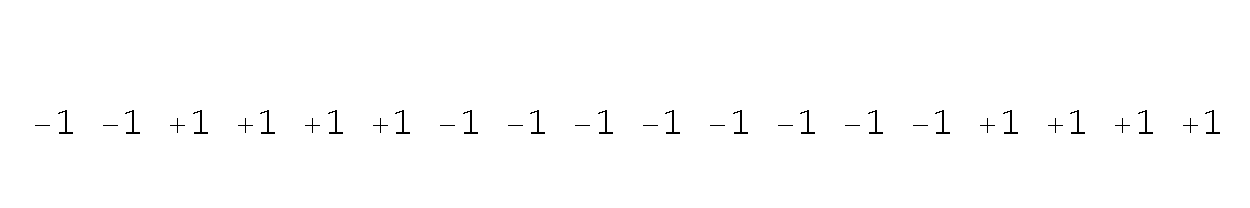
\includegraphics[width=\textwidth]{2 pseudosymbols.pdf}}%
    \only<2-3>{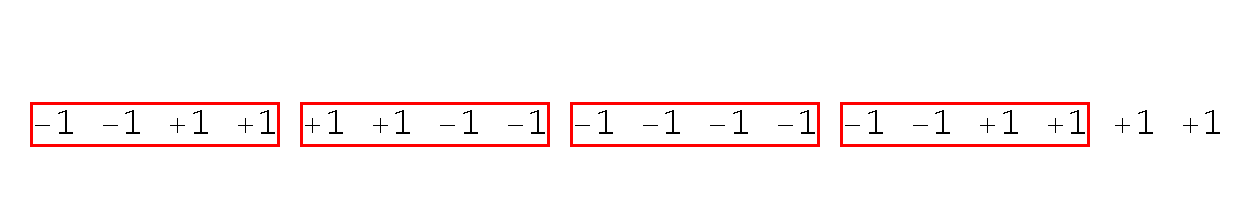
\includegraphics[width=\textwidth]{3 pseudosymbols.pdf}}%
    \only<4>{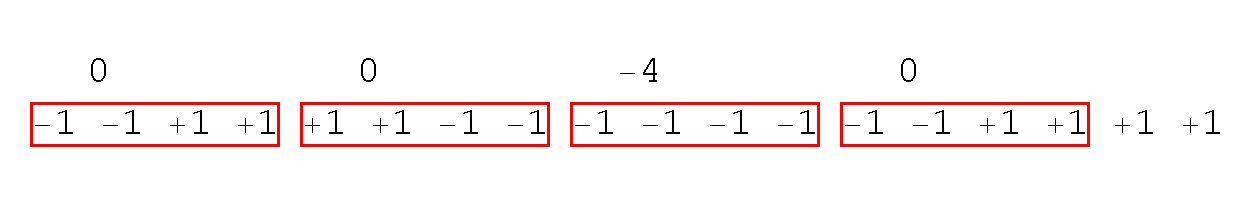
\includegraphics[width=\textwidth]{4 pseudosymbols.pdf}}%
    \only<5-6>{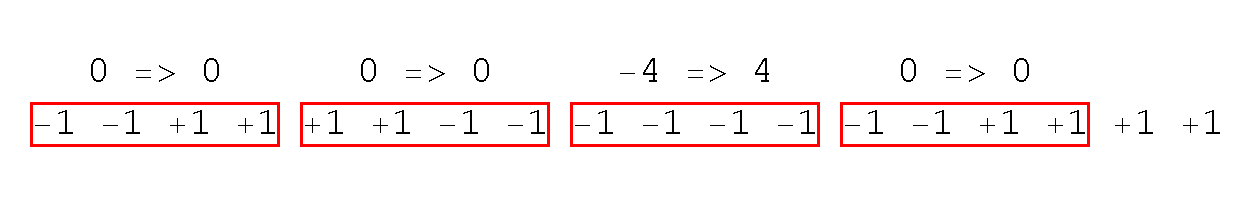
\includegraphics[width=\textwidth]{5 pseudosymbols.pdf}}%
    \only<7>{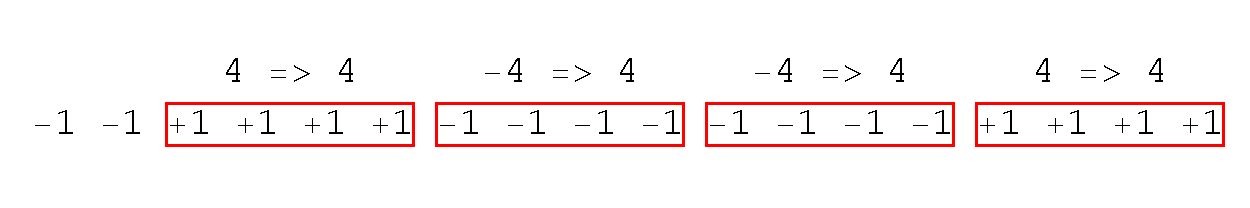
\includegraphics[width=\textwidth]{6 pseudosymbols.pdf}}%
    \only<8>{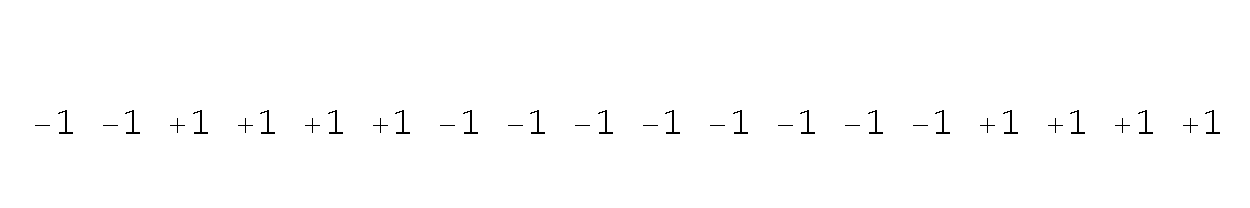
\includegraphics[width=\textwidth]{2 pseudosymbols.pdf}}%
    \only<9>{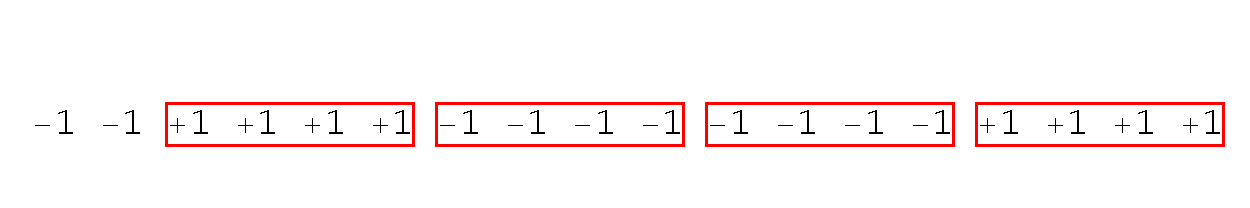
\includegraphics[width=\textwidth]{7 pseudosymbols.pdf}}%
    
    \onslide<3->{
        \begin{tabular}{r|r}
            Offset & Score \\
            \hline
            0 & \onslide<6->{1.0} \\
            1 & \onslide<8->{2.5} \\
            \only<-8>{2}\only<9>{\textbf{2}} & \only<7-8>{4.0}\only<9>{\textbf{4.0}} \\
            3 & \onslide<8->{2.6}
        \end{tabular}
    }
\end{frame}

\section{Pseudobit integration}

\begin{frame}
    \frametitle{Pseudobit integration}

    \centering
    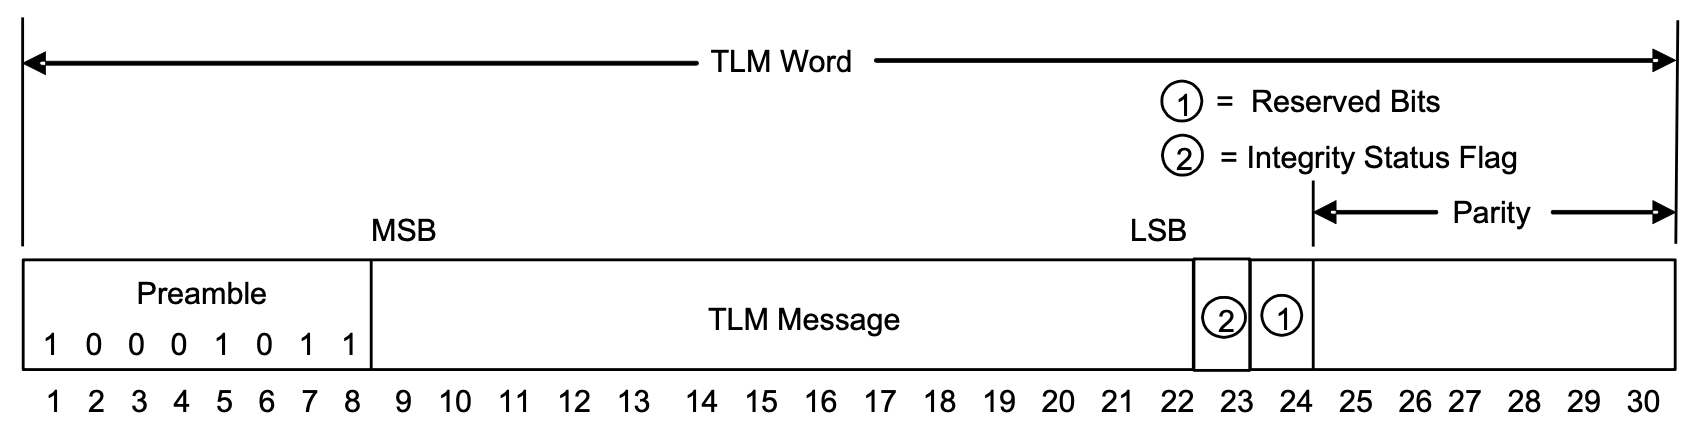
\includegraphics[width=\textwidth]{8 tlm word.png} \\
    \texttt{\tiny{Source: Figure 20-2, IS-GPS-200M, https://www.gps.gov/technical/icwg/IS-GPS-200M.pdf}}

    \vspace{0.5cm}

    \Large
    \onslide<2->{\texttt{-1 +1 +1 +1 -1 +1 -1 -1} $\Rightarrow$ $-1$ maps to $1$, $+1$ maps to $0$} \\
    \onslide<3->{\texttt{+1 -1 -1 -1 +1 -1 +1 +1} $\Rightarrow$ $+1$ maps to $1$, $-1$ maps to $0$}
\end{frame}

\section{Decoding subframes}

\begin{frame}
    \frametitle{Parity bits}

    \centering
    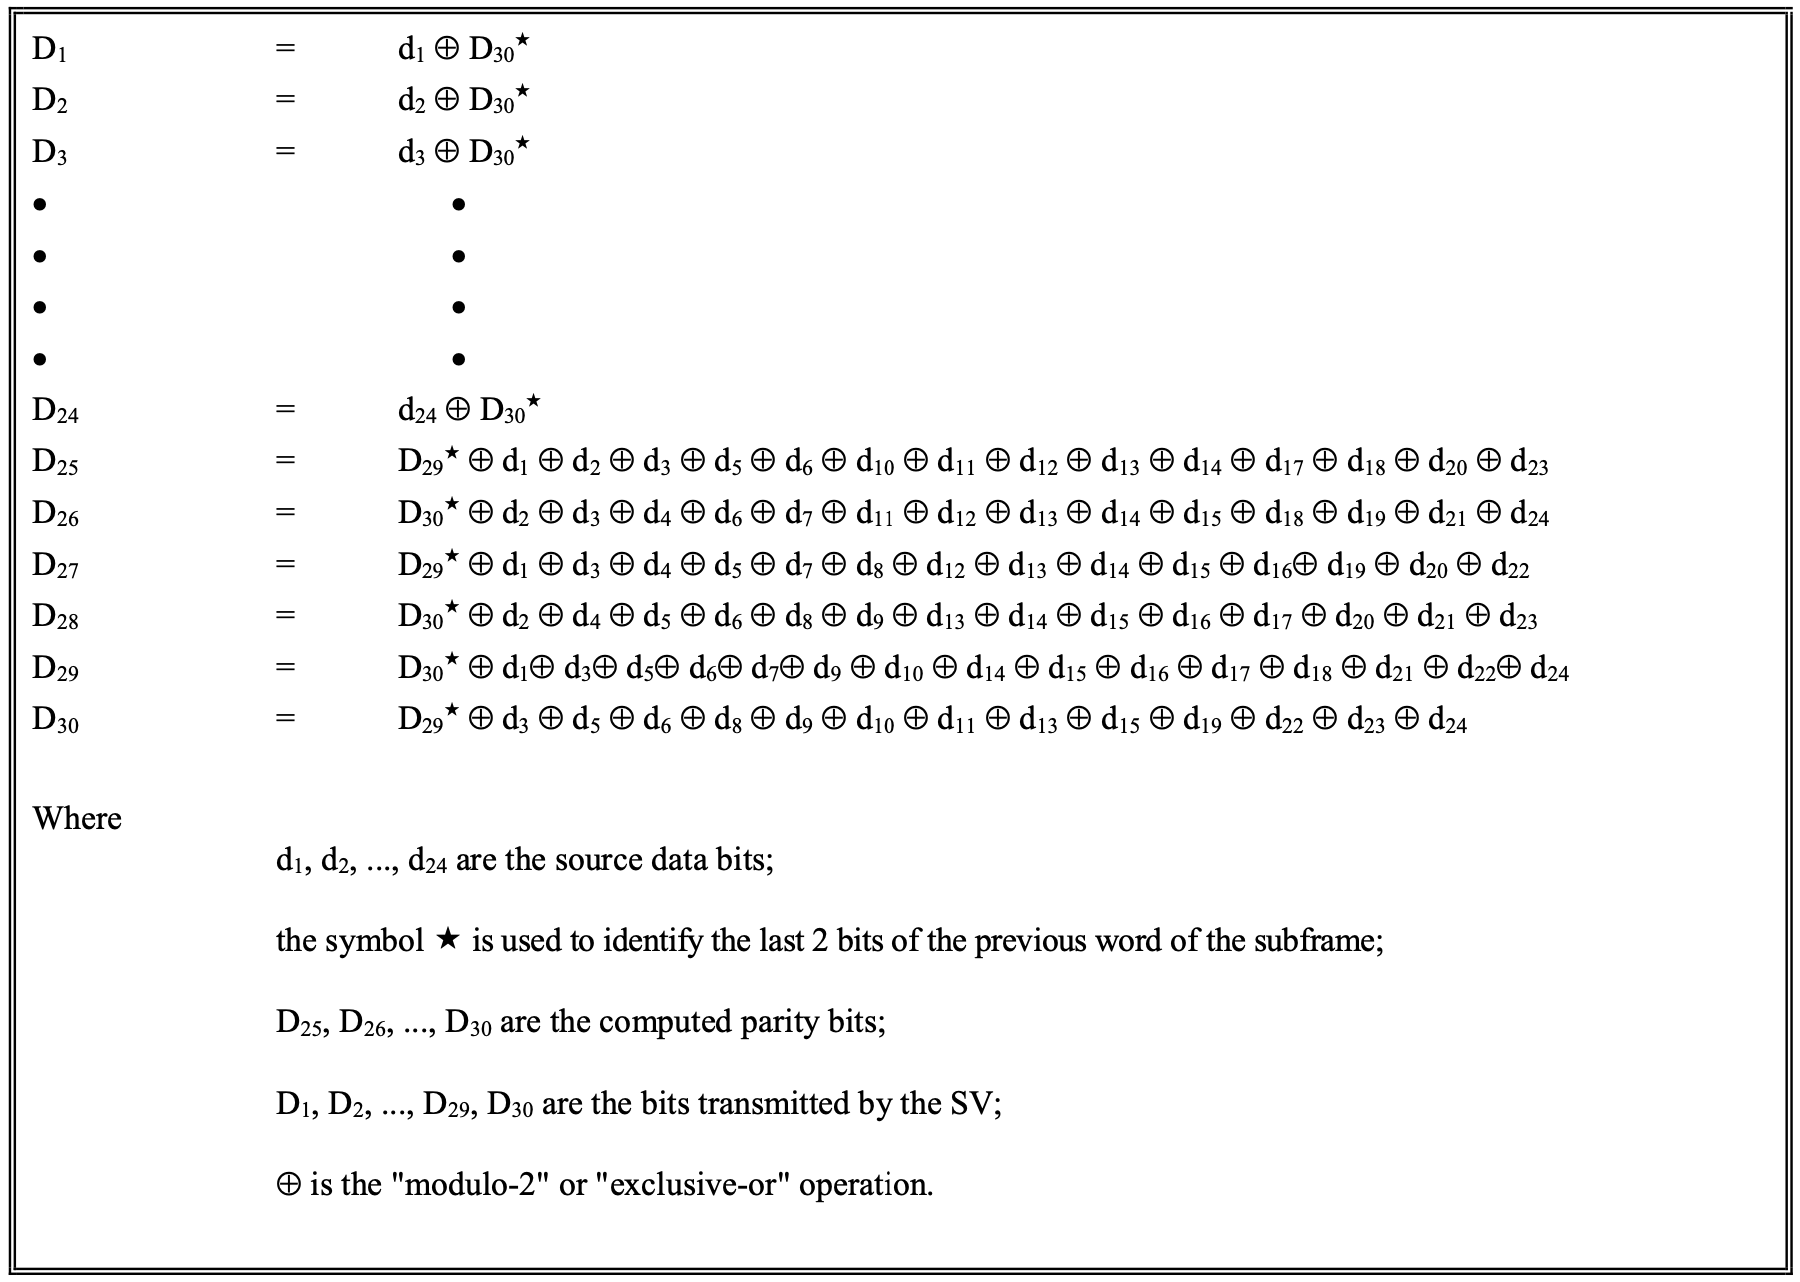
\includegraphics[width=\textwidth * 6 / 10]{9 parity equations.png} \\
    \texttt{\tiny{Source: Table 20-XIV, IS-GPS-200M, https://www.gps.gov/technical/icwg/IS-GPS-200M.pdf}}
\end{frame}

\begin{frame}
    \frametitle{The telemetry word}

    \centering
    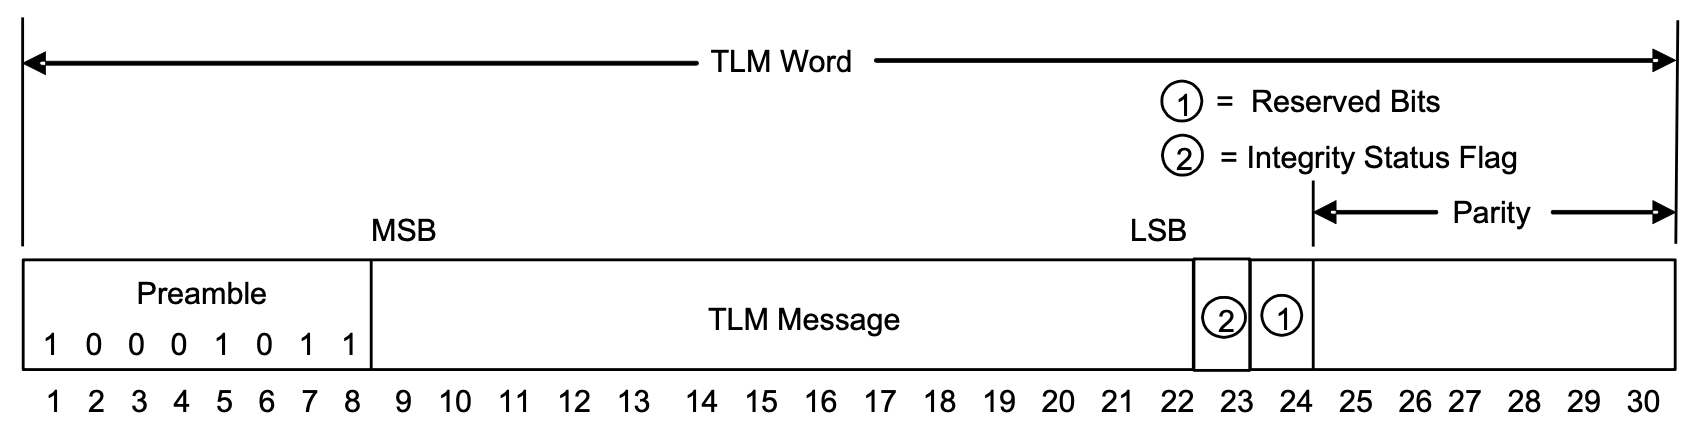
\includegraphics[width=\textwidth]{8 tlm word.png} \\
    \texttt{\tiny{Source: Figure 20-2, IS-GPS-200M, https://www.gps.gov/technical/icwg/IS-GPS-200M.pdf}}
\end{frame}

\begin{frame}
    \frametitle{The handover word}

    \centering
    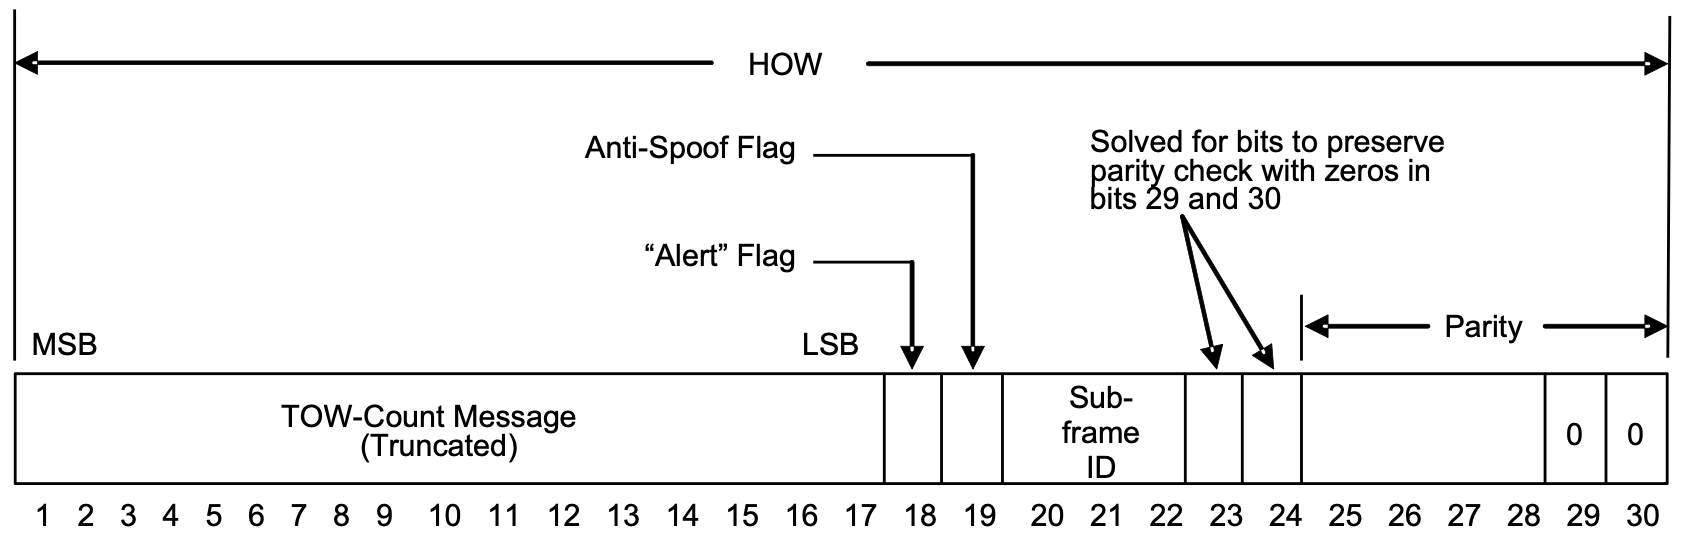
\includegraphics[width=\textwidth]{10 handover word.png} \\
    \texttt{\tiny{Source: Figure 20-2, IS-GPS-200M, https://www.gps.gov/technical/icwg/IS-GPS-200M.pdf}}
\end{frame}

\begin{frame}
    \frametitle{The TOW count}

    \begin{itemize}
        \item GPS started operating at midnight UTC on the night of Saturday January 5, 1980
        
        \item<2-> The number of weeks that have passed since that night is called the GPS week number
        
        \item<3-> The time-of-week count (TOW count) is the number of 1.5 s periods that have elapsed since the start of the current GPS week (since midnight UTC Saturday night)
        
        \item<4-> The TOW count is a 19 bit number
        
        \item<5-> The truncated TOW count is the 17 most significant bits of the TOW count as it will appear at the time the next subframe begins transmission
        
        \item<6-> This corresponds to a $\qty{6}{s}$ period — how long it takes to transmit a subframe — so the truncated TOW count will increment by 1 with each subframe we receive
        
        \item<7-> We can use this to calculate the signal's transmission time
    \end{itemize}
\end{frame}

\begin{frame}
    \frametitle{The handover word}

    \centering
    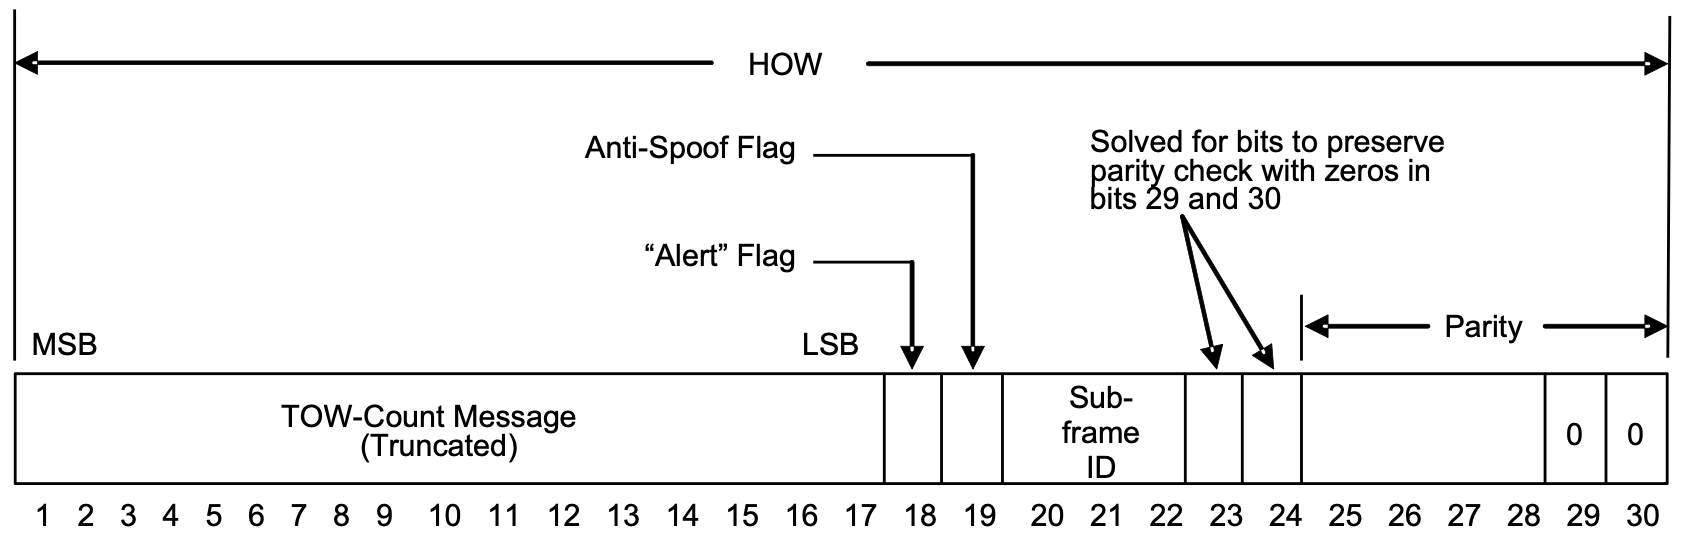
\includegraphics[width=\textwidth]{10 handover word.png} \\
    \texttt{\tiny{Source: Figure 20-2, IS-GPS-200M, https://www.gps.gov/technical/icwg/IS-GPS-200M.pdf}}
\end{frame}

\begin{frame}
    \frametitle{Subframes}

    \begin{itemize}
        \item<2-> Subframe 1
        
        \begin{itemize}
            \item<3-> Clock parameters
            
            \begin{itemize}
                \item<4-> Calculate when signals were transmitted
                
                \item<5-> Correct for atomic clock drift
            \end{itemize}
            
            \item<6-> Health information
        \end{itemize}

        \item<7-> Subframes 2 and 3
        
        \begin{itemize}
            \item<8-> Orbital parameters
            
            \begin{itemize}
                \item<9-> Calculate a satellite's position
            \end{itemize}
        \end{itemize}

        \item<10-> Subframes 4 and 5
        
        \begin{itemize}
            \item<11-> Parameters change every frame over 25 frames (12.5 minutes)
            
            \begin{itemize}
                \item<12-> Other satellites
                
                \item<13-> Earth's atmospheric conditions
                
                \item<14-> Etc.
            \end{itemize}
        \end{itemize}
    \end{itemize}
\end{frame}

\section{Decoding subframe parameters}

\begin{frame}
    \frametitle{Decoding numbers}

    \centering
    \only<1>{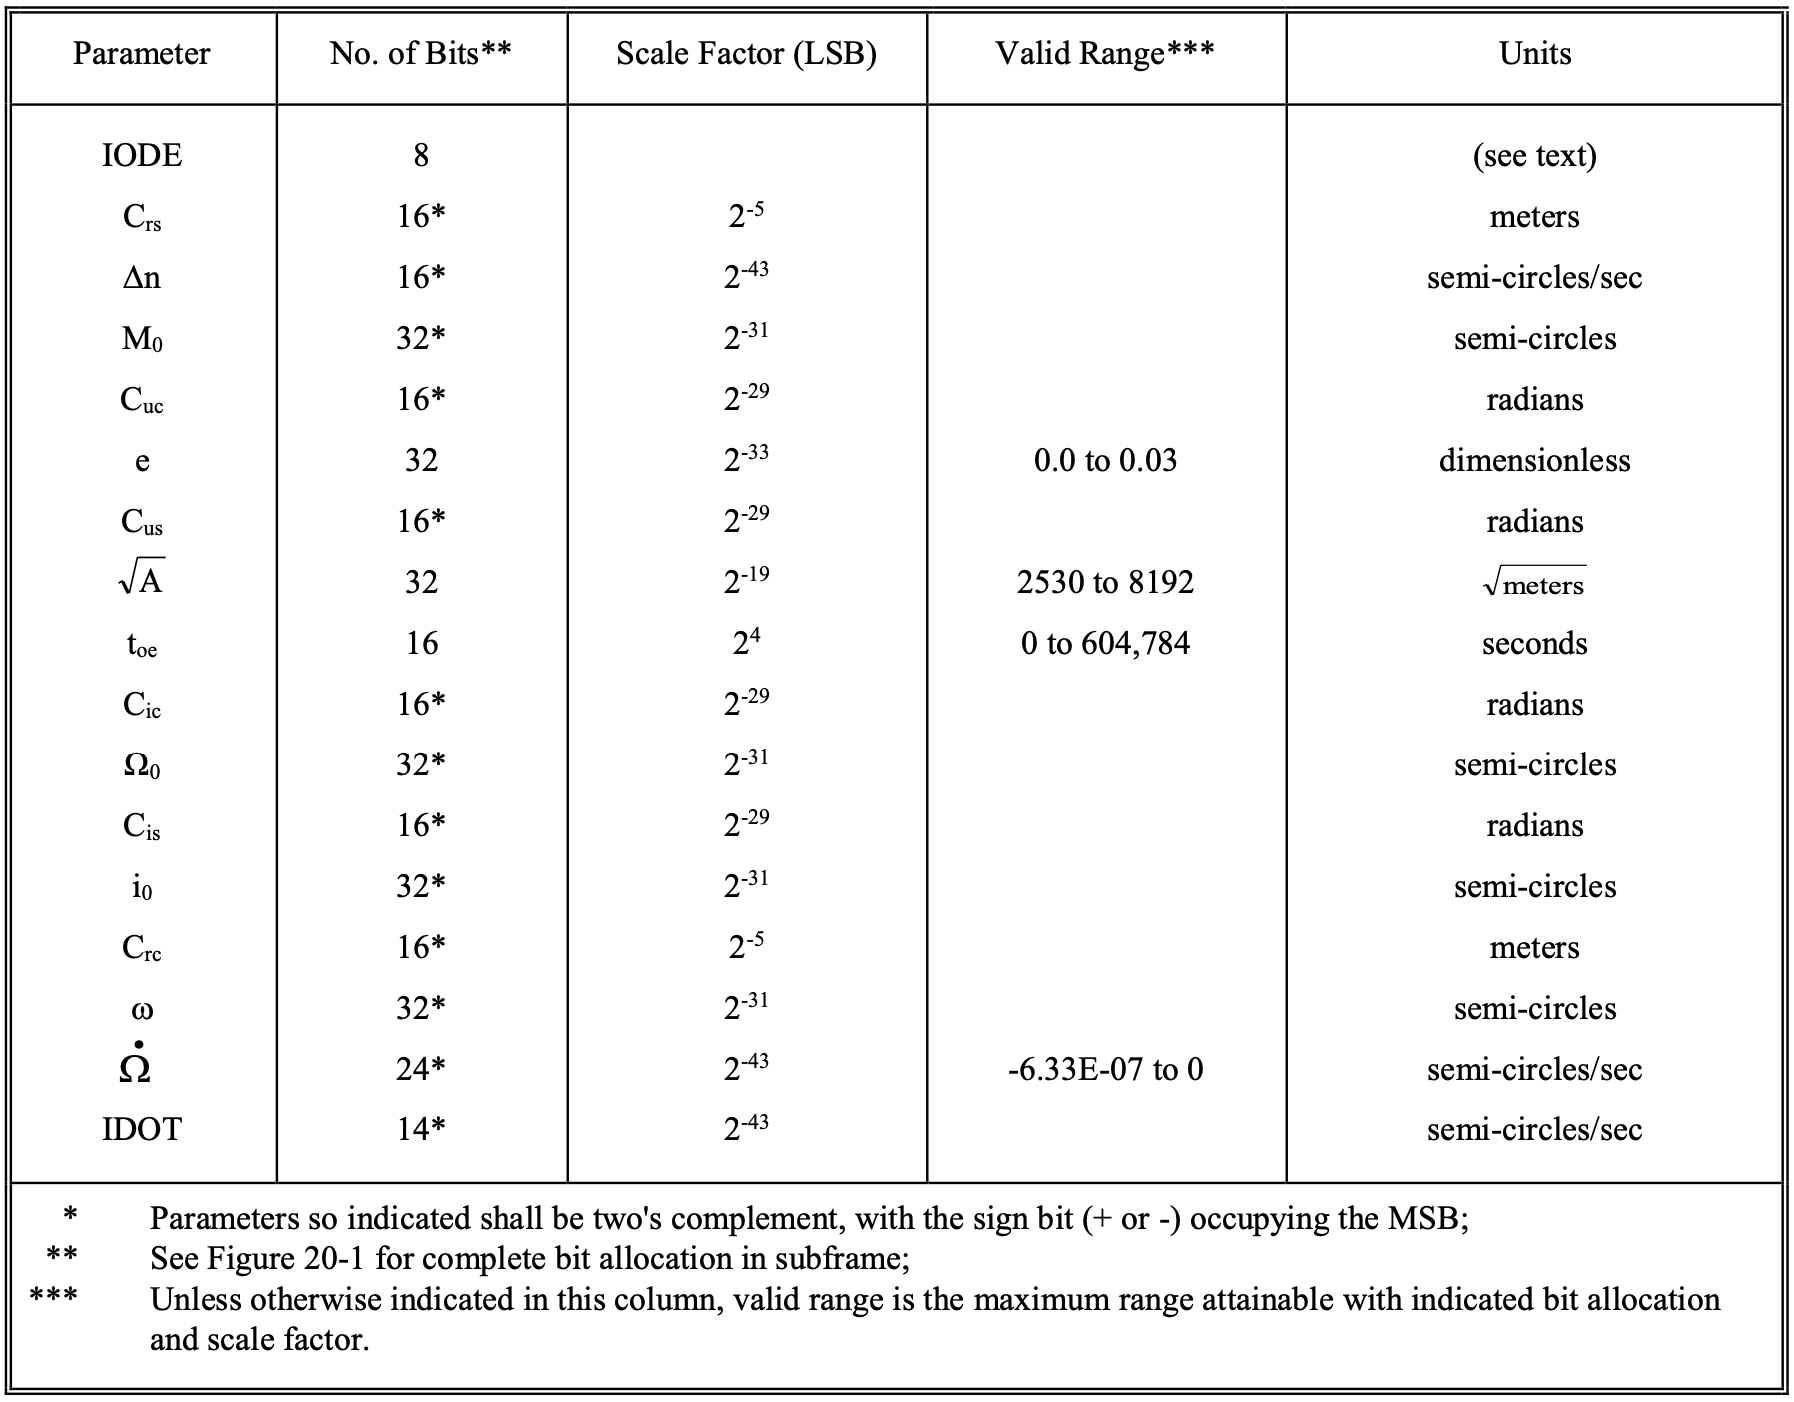
\includegraphics[width=\textwidth * 11 / 20]{11 numbers.png}}%
    \only<2>{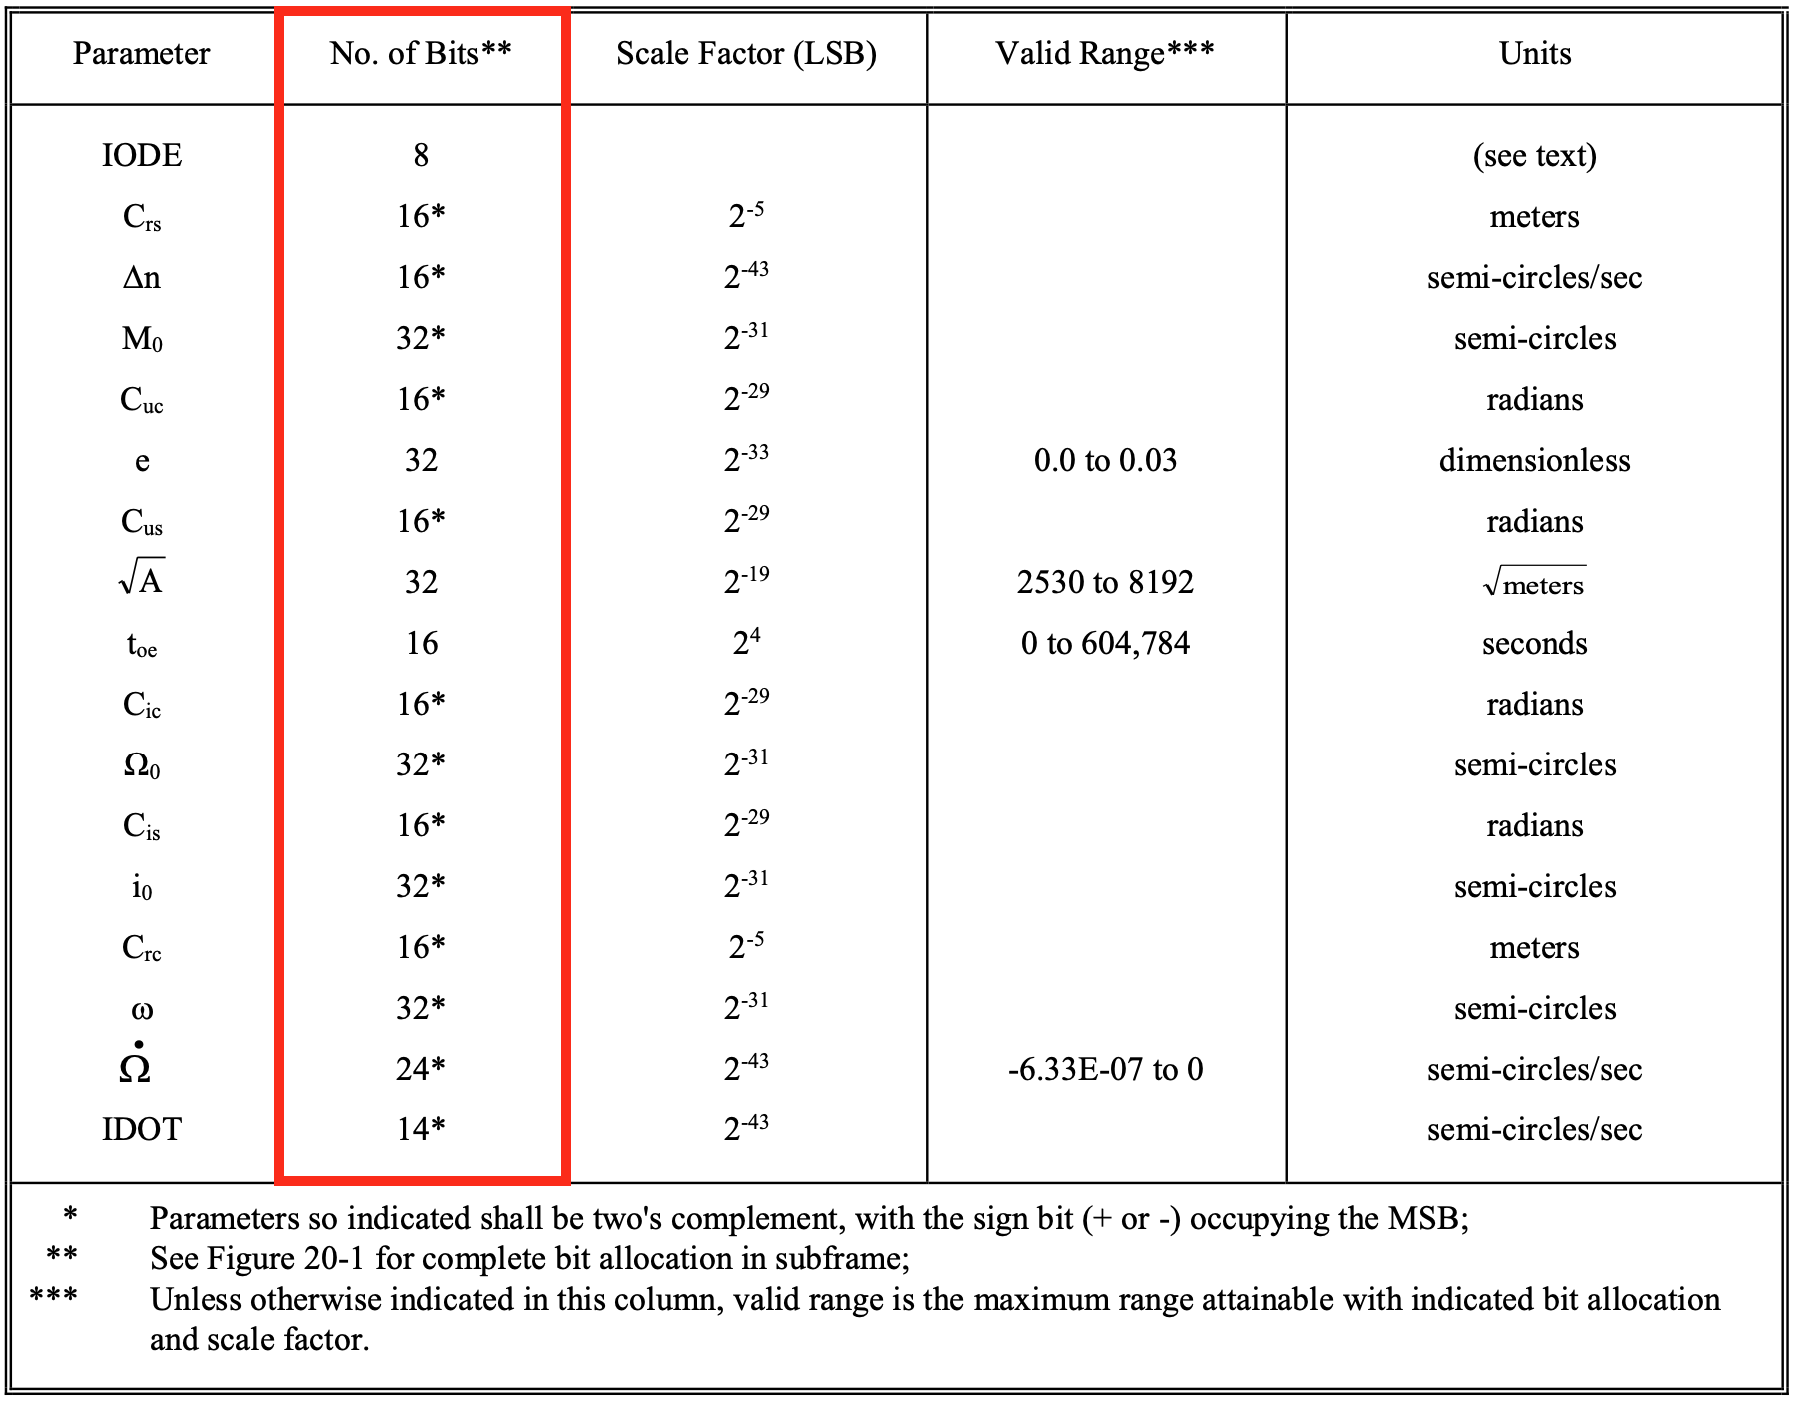
\includegraphics[width=\textwidth * 11 / 20]{12 numbers bits.png}}%
    \only<3>{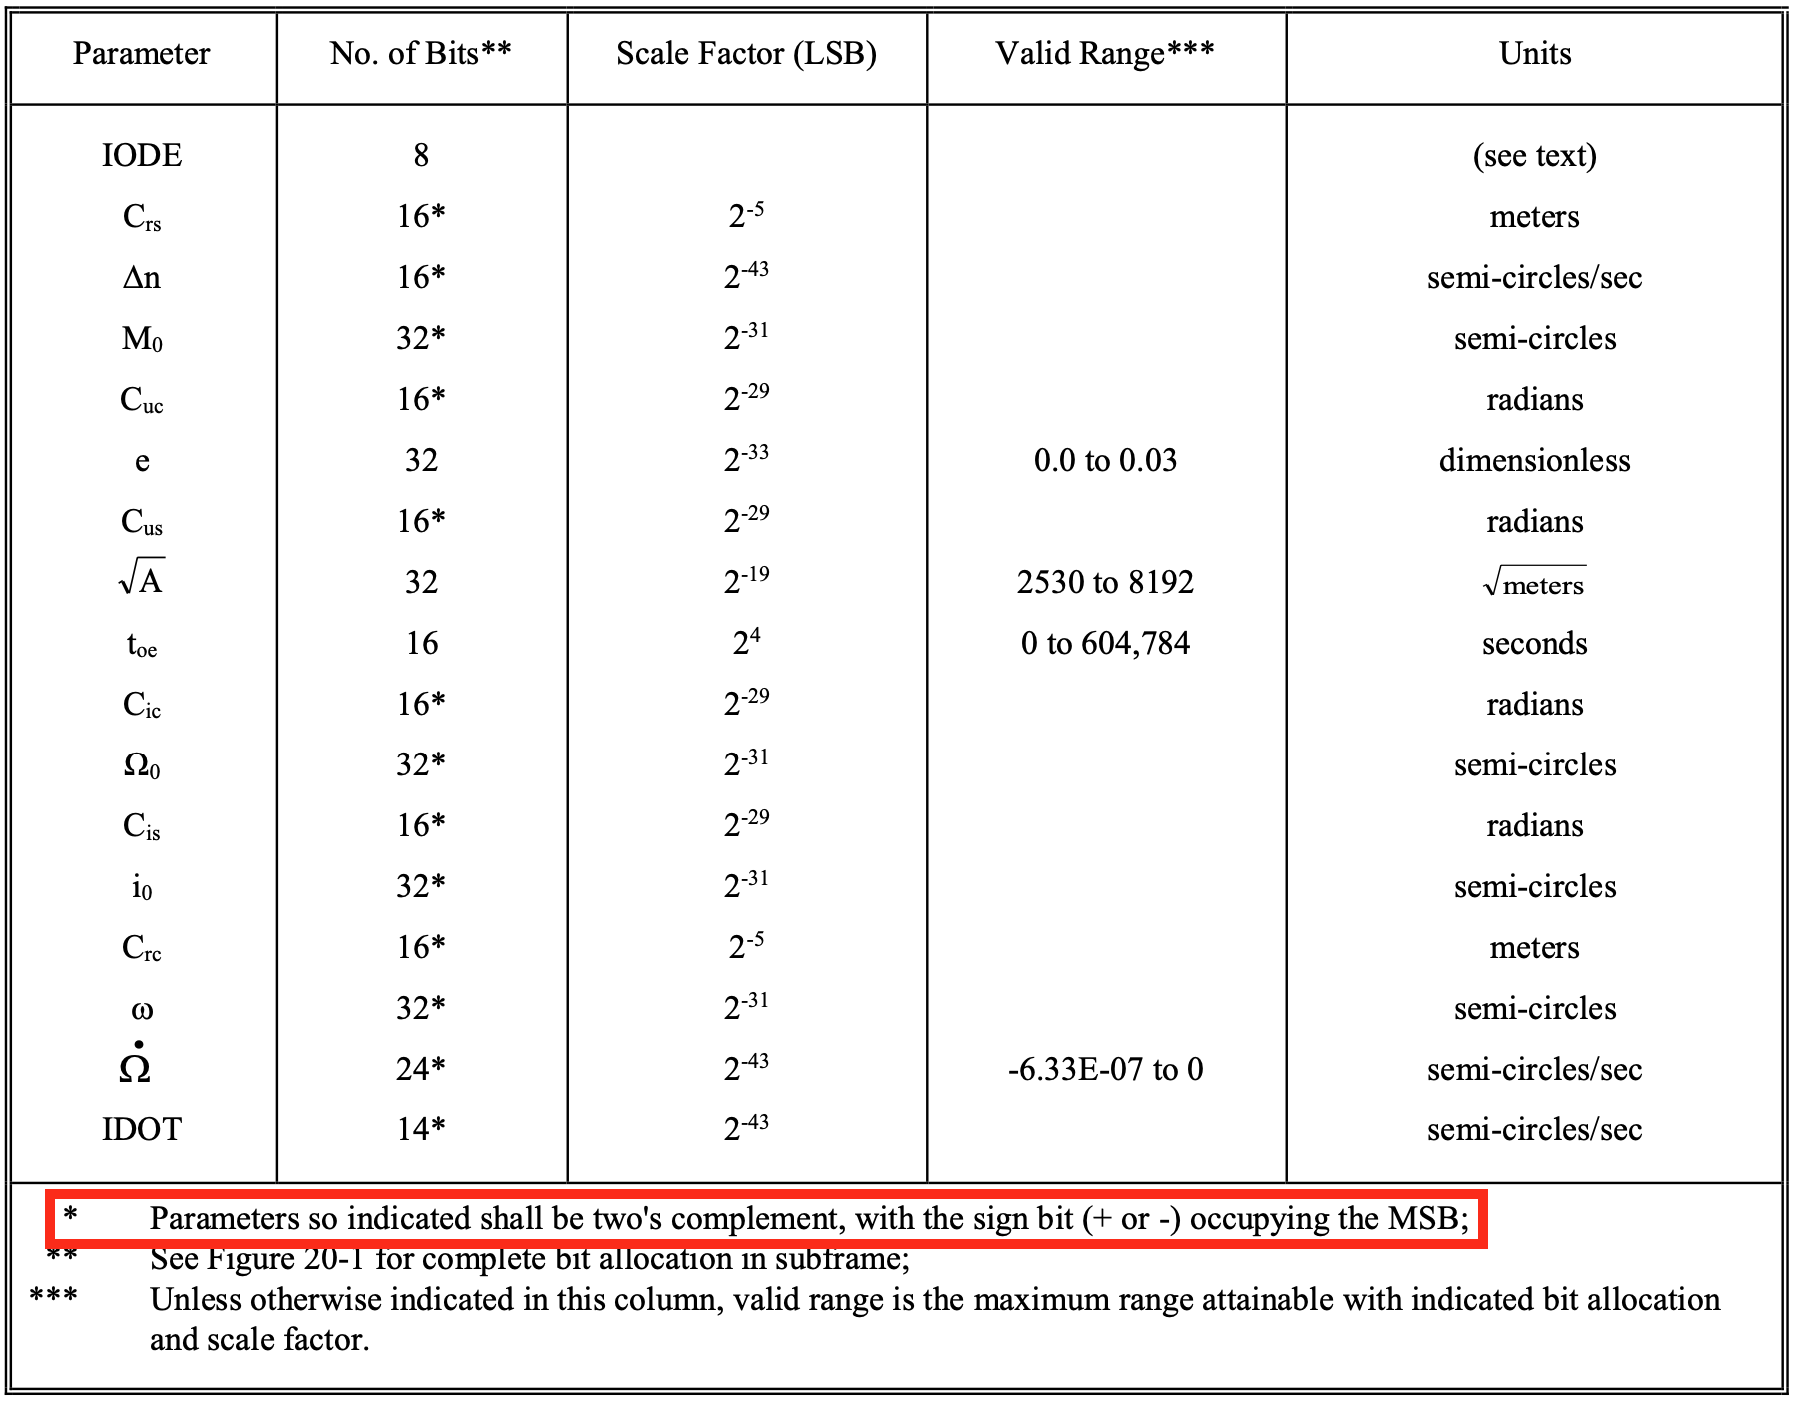
\includegraphics[width=\textwidth * 11 / 20]{13 numbers twos complement.png}}%
    \only<4>{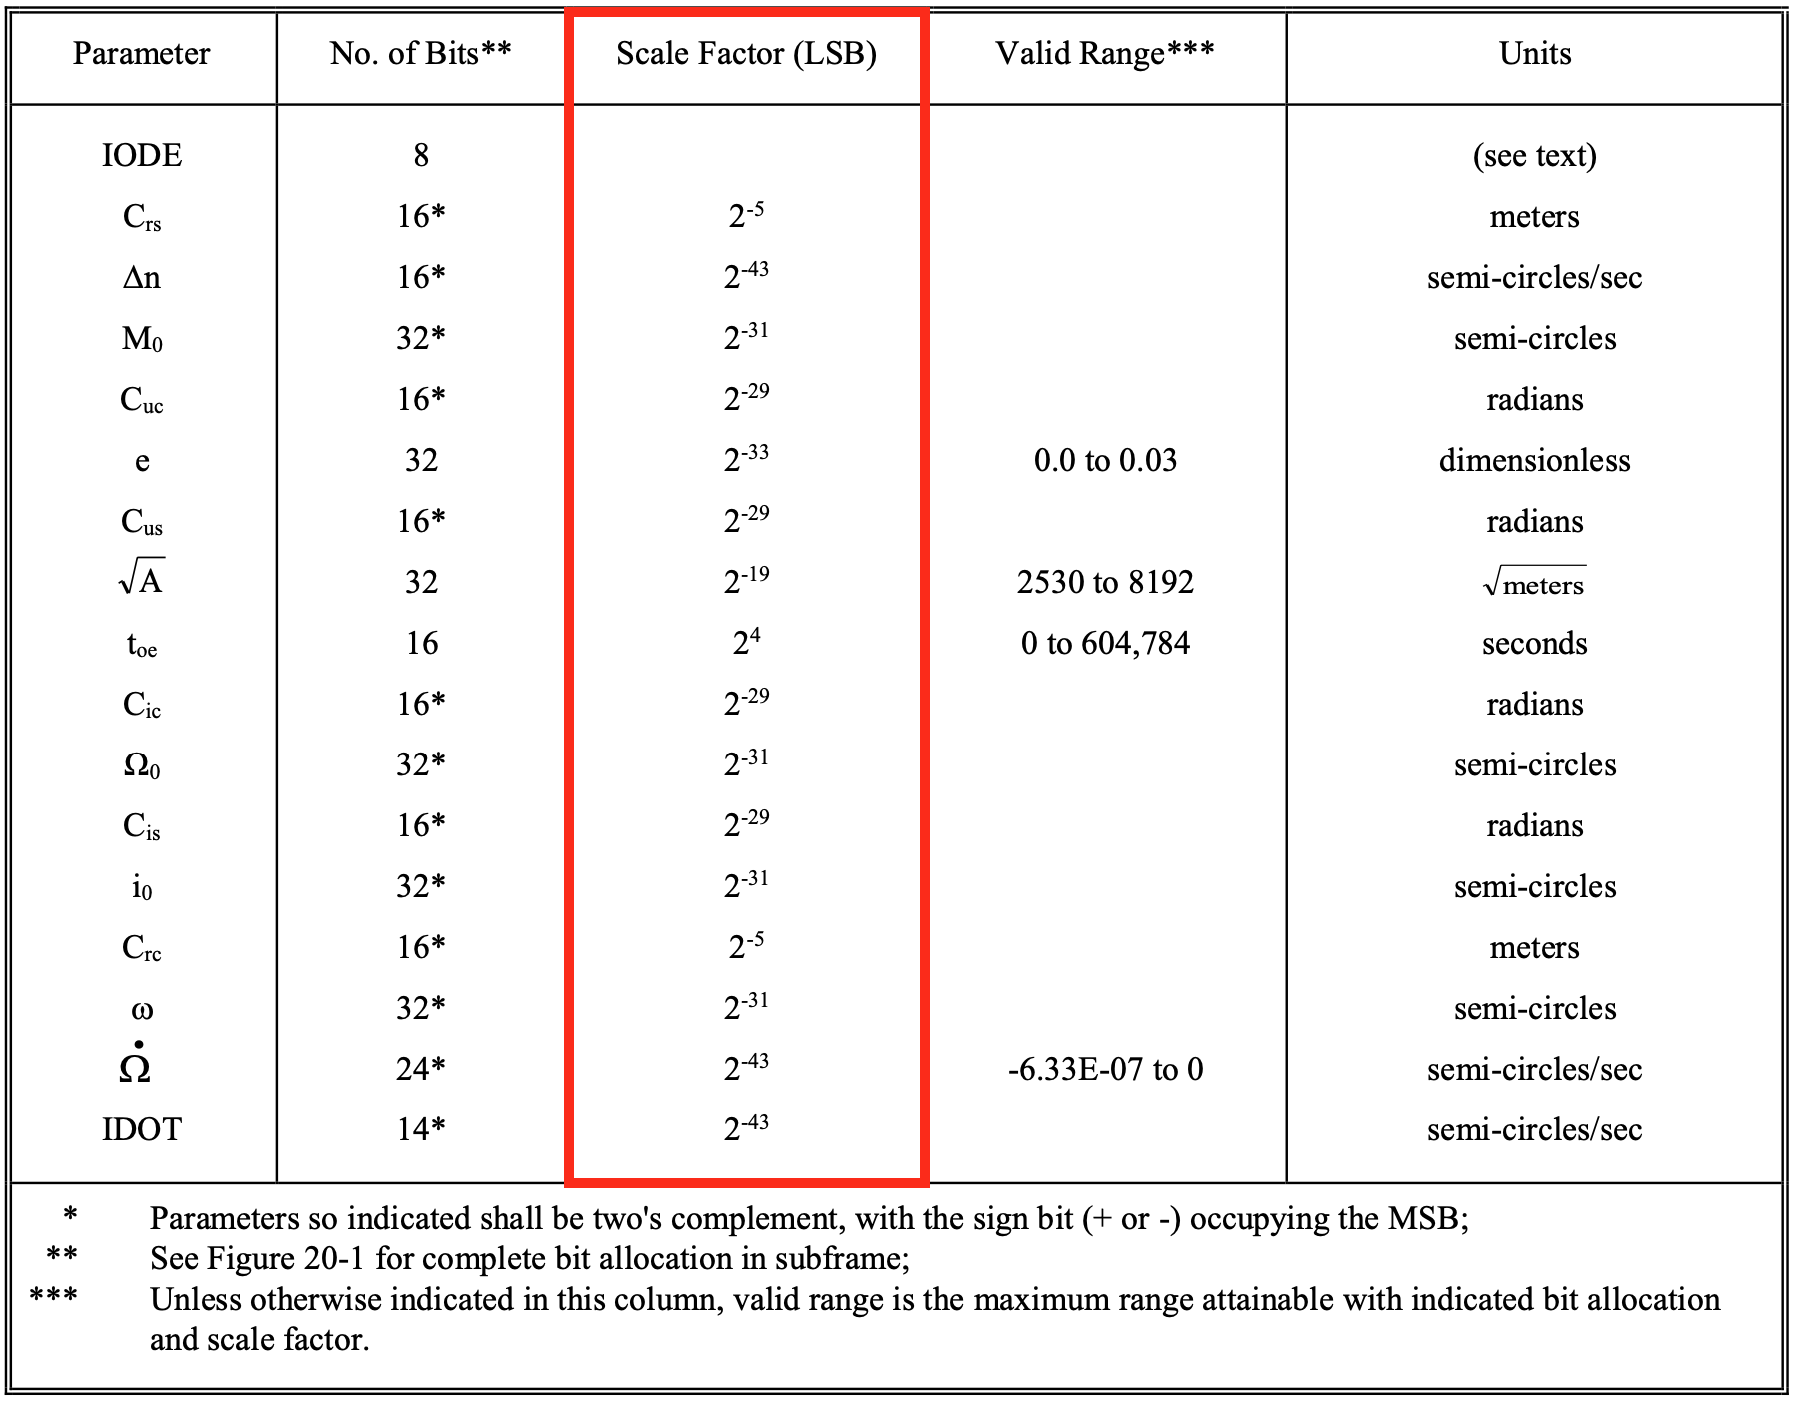
\includegraphics[width=\textwidth * 11 / 20]{14 numbers scale factor.png}}%
    \\ \texttt{\tiny{Source: Table 20-III, IS-GPS-200M, https://www.gps.gov/technical/icwg/IS-GPS-200M.pdf}}
\end{frame}

\begin{frame}
    \frametitle{Decoding numbers}

    \begin{enumerate}
        \item<2-> Parse the bits as if they were a normal integer

        \item<3-> Convert the integer from two's complement representation (if necessary)

        \item<4-> Multiply by the scale factor
    \end{enumerate}
\end{frame}

\begin{frame}
    \frametitle{Decoding numbers}

    \centering
    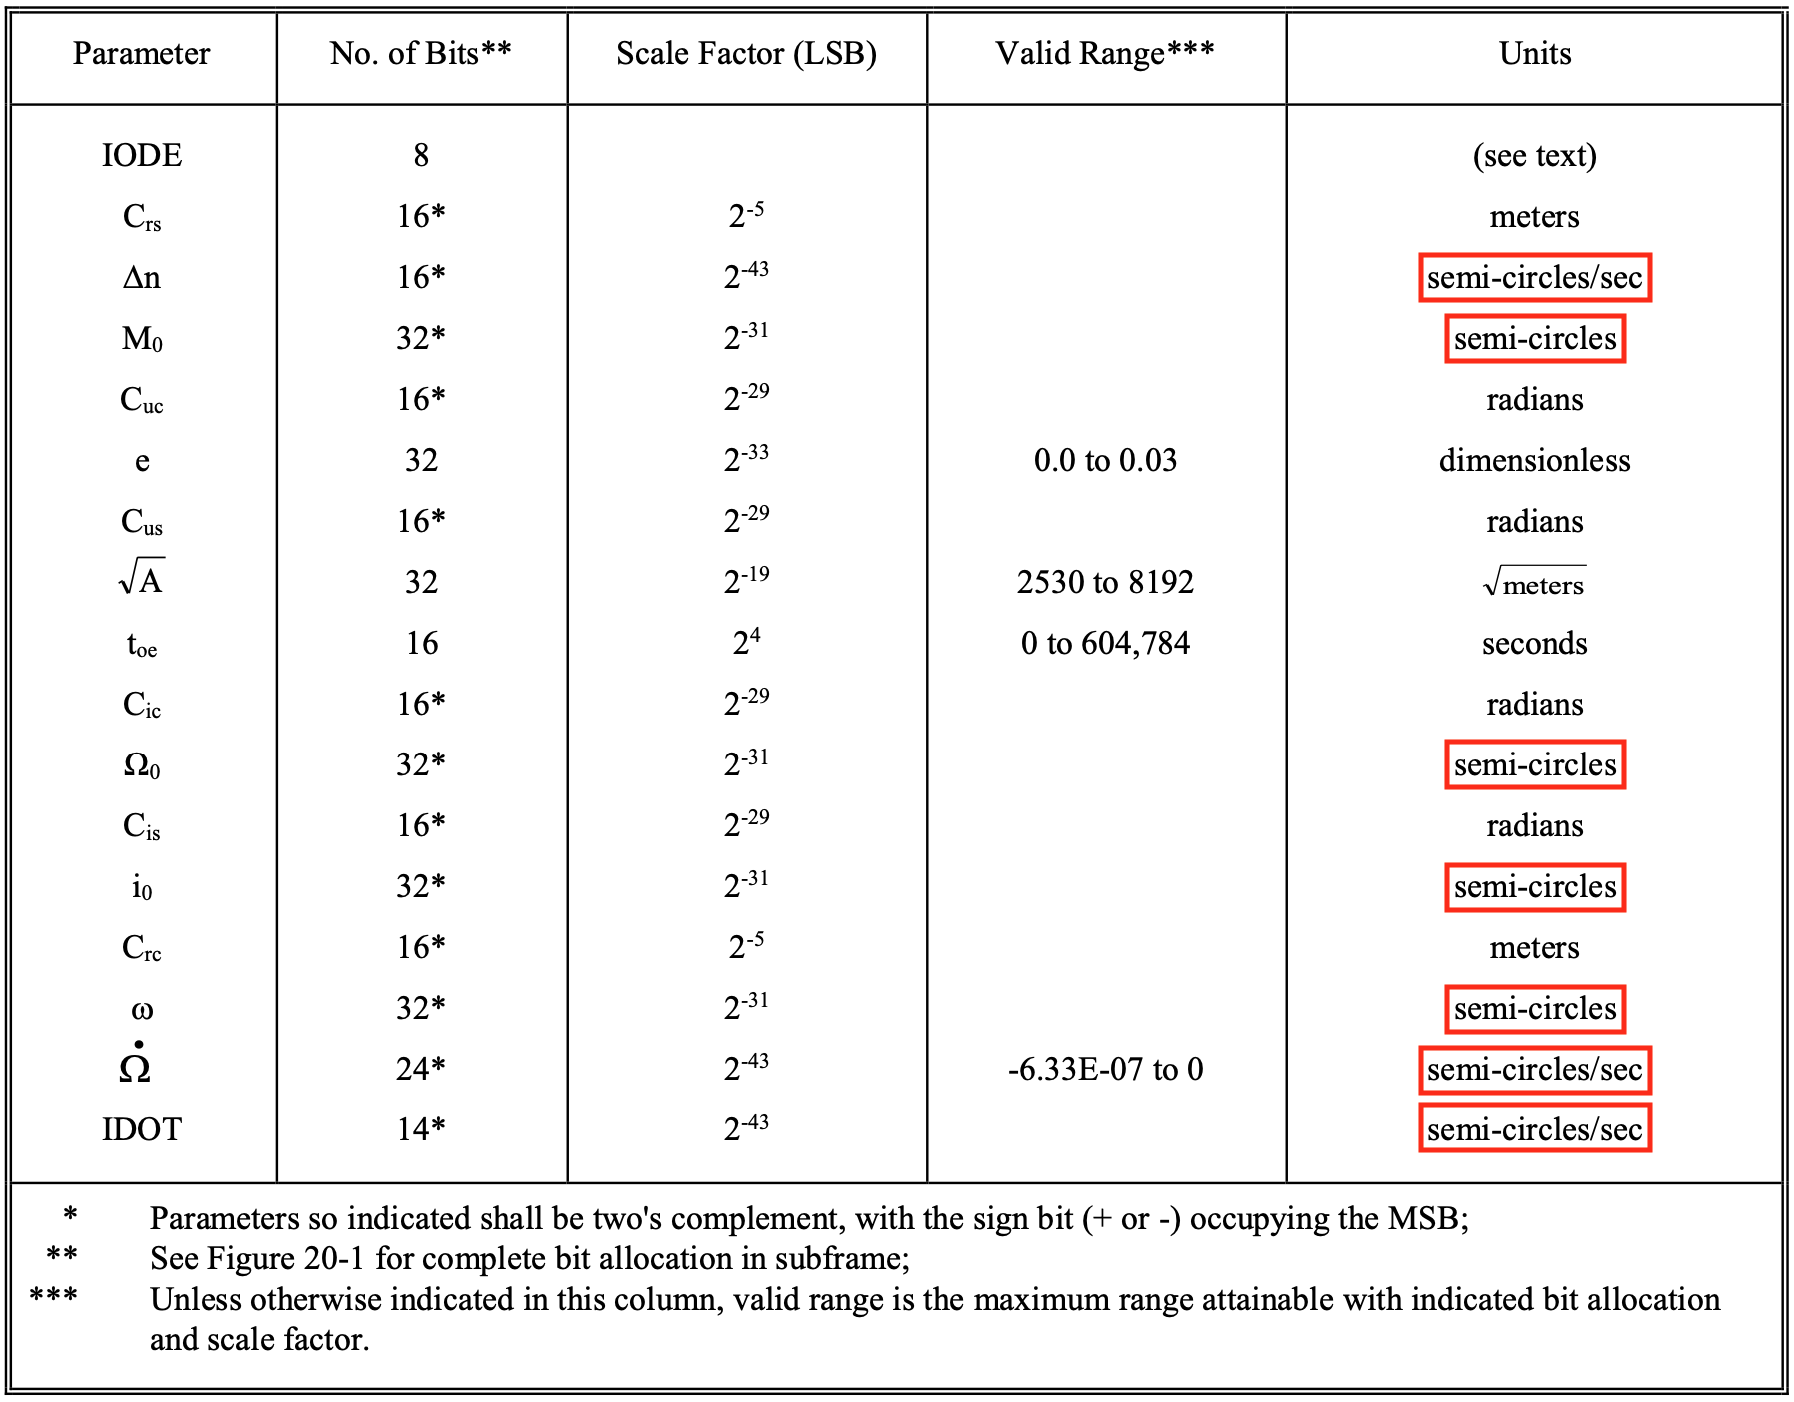
\includegraphics[width=\textwidth * 11 / 20]{15 numbers semi-circles.png} \\
    \texttt{\tiny{Source: Table 20-III, IS-GPS-200M, https://www.gps.gov/technical/icwg/IS-GPS-200M.pdf}}
\end{frame}

\begin{frame}
    \frametitle{Recap}

    \begin{itemize}
        \item<2-> Pseudosymbols $\rightarrow$ bits $\rightarrow$ words $\rightarrow$ subframes $\rightarrow$ frames
        
        \item<3-> Group pseudosymbols into pseudobits

        \begin{enumerate}
            \item<4-> Collect several bits worth of pseudosymbols

            \item<5-> Calculate a score for each possible grouping

            \item<6-> Choose the one with the greatest score
        \end{enumerate}

        \item<7-> Map pseudobits to bits

        \begin{enumerate}
            \item<8-> Collect several subframes worth of pseudobits

            \item<9-> Search for the telemetry word preamble (or its inverse)
        \end{enumerate}

        \item<10-> Obtain subframes' data bits by applying the parity algorithm
        
        \item<11-> TOW count in handover word tells when the next subframe begins transmission

        \item<12-> Different subframes contain different parameters — we need 1, 2, and 3
    \end{itemize}
\end{frame}

\end{document}